\documentclass{article}


\usepackage{arxiv}

\usepackage[utf8]{inputenc} % allow utf-8 input
\usepackage[T1]{fontenc}    % use 8-bit T1 fonts
\usepackage{hyperref}       % hyperlinks
\usepackage{url}            % simple URL typesetting
\usepackage{booktabs}       % professional-quality tables
\usepackage{amsfonts}       % blackboard math symbols
\usepackage{nicefrac}       % compact symbols for 1/2, etc.
\usepackage{microtype}      % microtypography
\usepackage{lipsum}
\usepackage{graphicx}
\usepackage{amsmath}
\graphicspath{ {./images/} }


\title{Point cloud classification using deep neural networks}


\author{
 Federica Di Lauro \\
  829470\\
  \texttt{f.dilauro2@campus.unimib.it} \\
  %% examples of more authors
   \And
  Andrea Premate \\
  829777\\
  \texttt{a.premate@campus.unimib.it} \\
  \And
  Lidia Lucrezia Tonelli \\
  813114\\
  \texttt{l.tonelli@campus.unimib.it} \\
}

\begin{document}
\maketitle
\begin{abstract}
TODO
\end{abstract}

\section{Introduction}

\cite{lu2020deep}

\paragraph{Point Cloud}

\paragraph{Classification task}

\paragraph{Dataset}

ModelNet40 \cite{ShapeNets}

\paragraph{Metrics}

\section{Classification Methods}

\subsection{Projection based}

\subsubsection{Multi-View}
\subsubsection{Volumetric}

\subsection{Point Based}

\subsubsection{Multi Layer Perceptron}


\newpage %TODO togliere newpage, è solo per regolarmi
\subsubsection{Convolutional Neural Networks}
The convolution operator is defined on two functions $f(\mathbf{x})$ and $g(\mathbf{x})$, with $\mathbf{x} \in \mathbb{R}^{d}$: 

\begin{equation}
    (f * g)(\mathbf{x})=\iint_{\boldsymbol{\tau} \in \mathbb{R}^{d}} f(\boldsymbol{\tau}) g(\mathbf{x}+\boldsymbol{\tau}) d \boldsymbol{\tau}
\end{equation}

In images the function $g(\mathbf{x})$ is a 2D function, and because images are made up by a discrete and fixed grid of pixel the integrals can be seen as the discrete sum of product between $f$ and $g$.

Such a regular structure is not intrinsic of point clouds, and thus convolution is not as easily implemented.

To tackle this problem without using an intermediate representation of the point cloud (as seen with projection based approaches) specialized convolution operators have been proposed.

In this section the PointConv operation, proposed by Wenxuan Wu et al~\cite{PointConv}, will be explored.

\paragraph{PointConv}

A point cloud is a set of 3D points $(x,y,z)$, so the 3D convolution can be written as: 

\begin{equation}
    \begin{array}{l}
\operatorname{Conv}(W, F)_{x y z}= 
\quad \iiint_{\left(\delta_{x}, \delta_{y}, \delta_{z}\right) \in G} W\left(\delta_{x}, \delta_{y}, \delta_{z}\right) F\left(x+\delta_{x}, y+\delta_{y}, z+\delta_{z}\right) d \delta_{x} d \delta_{y} d \delta_{z}
\end{array}
\end{equation}

where $W(\delta_{x}, \delta_{y}, \delta_{z})$ is the weight function and $F\left(x+\delta_{x}, y+\delta_{y}, z+\delta_{z}\right)$ is the feature of a point in the local region $G$ centered in  $p = (x,y,z)$.

Point clouds, unlike images, are not uniformly sampled from the 3D space: the points $(\delta_{x}, \delta_{y}, \delta_{z})$ do not have a fixed structure in the local region, so there could be subregions with more dense sampling and subregions with more sparse points, thus transforming the integral into a discrete sum is not trivial.
To deal with the uneven sampling the authors introduced the inverse sparsity function $S(x,y,z)$. The PointConv operator is thus defined as:

\begin{equation}
    \operatorname{PointConv} (S, W, F)_{x y z}=
\sum_{\left(\delta_{x}, \delta_{y}, \delta_{z}\right) \in G} S\left(\delta_{x}, \delta_{y}, \delta_{z}\right) W\left(\delta_{x}, \delta_{y}, \delta_{z}\right) F\left(x+\delta_{x}, y+\delta_{y}, z+\delta_{z}\right)
\end{equation}

Since the weights are shared between all the points, and that PointConv is a full approximation of a convolutional layer it is both invariant to permutation of the points and to translation.

The full structure of the PointConv operator, applied on a local region with $K$ points, can be seen in figure~\ref{fig:pointconvOperator}.

\begin{figure}[ht]
    \centering
    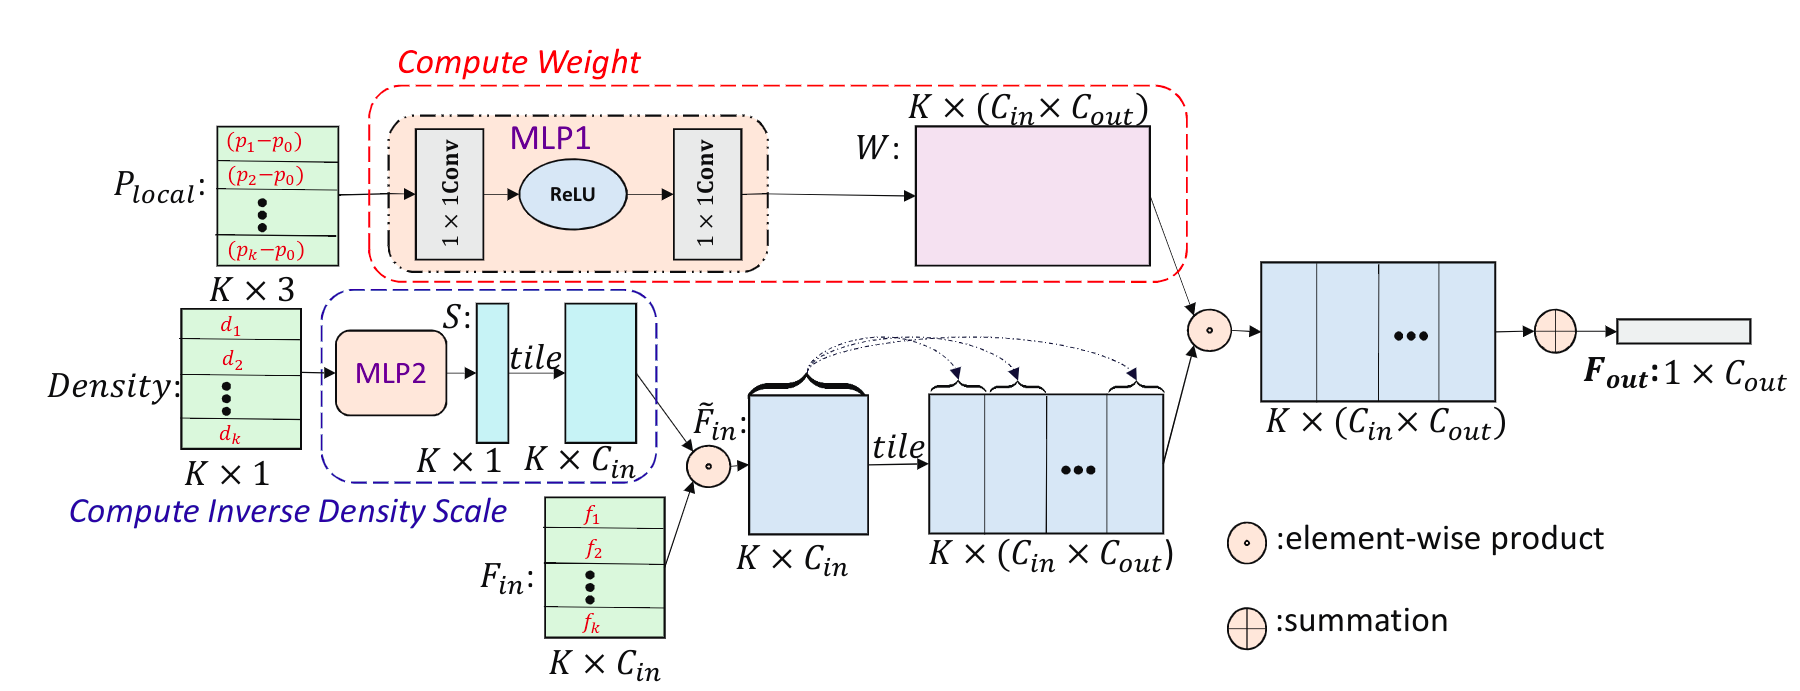
\includegraphics[width=\textwidth]{pointconv.png}
    \caption{PointConv operator~\cite{PointConv}}
    \label{fig:pointconvOperator}
\end{figure}

The weight function $W$ can be approximated by MLPs, while the density function, which outputs a value indicating how much points are concentrated around the centroid region, is calculated using kernel density estimation (KDE), described in~\cite{Turlach_bandwidthselection}, and then by appling a non-linear transform using an MLP.

The inputs of the PointConv operator are:

\begin{itemize}
    \item The subset of points $P_{local} \in \mathbb{R}^{K \times 3}$ : given a point $p_0$ in the point cloud, the $K$ closest points are taken and then the $p_0$ coordinates are subtracted to each point, obtaining the local coordinates of each point.
    \item The $ Density \in \mathbb{R} ^{K}$ estimated at each local point using KDE.
    \item The features $F_{in} \in \mathbb{R}^{K \times C_{in}}$, where $C_{in}$ is the number of channels, and for each channel there are the features associated with each local point. These features can be the point coordinates $(x, y, z)$, but also other features associated with the point such as the RGB color.
\end{itemize}

The \textit{Compute Weight} module is made by an MLP implemented as a $1 \times 1$ convolution, followed by a non-linear ReLU activation function, followed by another $1 \times 1$. The output of this module is $W \in \mathbb{R}^{K \times (C_{in} \times C_{out}})$.

The \textit{Compute Inverse Density Scale} module is used to calculate $S$: this is done by feeding the $Density$ into an MLP for a one dimensional linear transform. In this way the network can "decide" to use the density estimates.

Finally, the $F_{out} \in \mathbb{R}^{C_{out}}$ feature(s) associated with the feature(s) $F_{in}$ is:

\begin{equation}\label{eq:pointconv_orig}
\mathbf{F}_{\text {out }}=\sum_{k=1}^{K} \sum_{c_{i n}=1}^{C_{i n}} S(k) \mathbf{W}\left(k, c_{i n}\right) F_{i n}\left(k, c_{i n}\right)
\end{equation}

\paragraph{Architecture of a NN using PointConv} The architecture proposed in combination with PointConv is a hierarchical structure, composed by \textit{feature encoding blocks}. In each feature encoding block there is a sampling layer, a grouping layer and a PointConv. This feature encoding blocks (apart from the PointConv operator) are very similar to the ones already seen in PointNet++~\cite{qi2017pointnet++}, see also paragraph~\ref{par:pointnet++}. The only difference is that the neighbors of the centroid are calculated using the k-NN approach. In total the neural network is composed of 3 feature encoding blocks followed by 3 fully connected layers\footnote{See the code hosted on GitHub: \url{https://github.com/DylanWusee/pointconv_pytorch/blob/master/model/pointconv.py}}.

\paragraph{Efficient PointConv} A noticeable problem of the original PointConv operator is the memory needed for the $W$ function: given the batch size $B$, the number of points in the point cloud $N$, the number of local points $K$, the number of input channels $C_{in}$ and the number of output channels $C_{out}$ the size of the filter weight would be $B \times N \times K \times C_{in} \times C_{out}$.

It can be shown that PointConv equation~\ref{eq:pointconv_orig} can be reduced to a matrix multiplication and a 2D convolution. The new operator can be seen in figure~\ref{fig:efficientPointconv}. This can reduce the memory consumption by a factor of $1 / 64$.

\begin{figure}[ht]
    \centering
    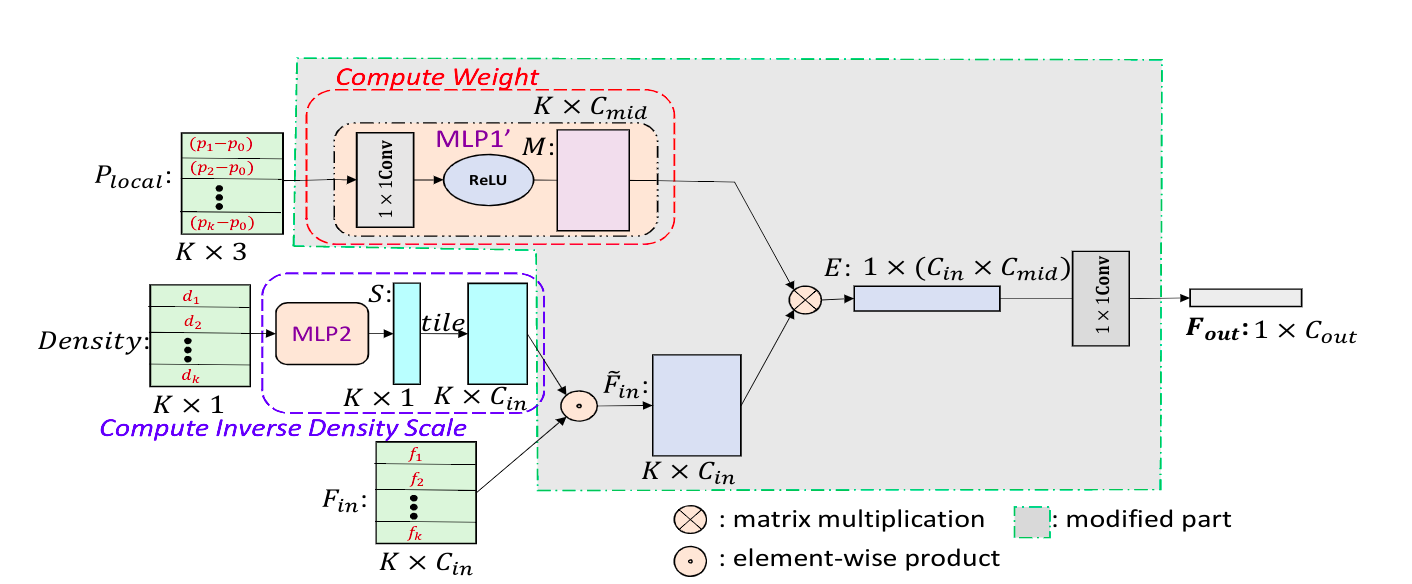
\includegraphics[width=\textwidth]{efficient_pointconv.png}
    \caption{Efficient PointConv~\cite{PointConv}}
    \label{fig:efficientPointconv}
\end{figure}

\paragraph{PointConv experiments}

The experiments have been performed on the ModelNet40 dataset, and have been conducted in the same way as PointNet authors did, which have become a standard to have a meaningful comparison between different networks. The overall accuracy obtained by PointConv on this dataset is $92.5$

An interesting experiment that has been carried out is the classification of CIFAR-10 dataset~\cite{Krizhevsky09learningmultiple}, which consists of 60000 32x32 colour images in 10 classes, with 6000 images per class. To demonstrate that PointConv is a good approximation of convolution the authors converted each point in an image into $(x,y)$ coordinates with the associated RGB color. Two CNNs have been trained, using PointConv as the convolution operator. The accuracy results in table~\ref{tab:pointconv_exp_cifar10} show that the networks using PointConv have roughly the same accuracy as normal CNNs, given that the overall architecture remains the same.

\begin{table}[ht]
    \centering
    \caption{CIFAR-10 experiments}
    \begin{tabular}{cc}
        \hline \text { Network } & \text { Accuracy (\%) } \\
        \hline AlexNet~\cite{AlexNet} & 89.00 \\
        VGG19~\cite{vgg19} & 93.60 \\
        \hline
        PointConv (5-layers) & 89.13 \\
        PointConv (VGG19) & 93.19 \\
        \hline
    \end{tabular}
    \label{tab:pointconv_exp_cifar10}
\end{table}

\newpage %TODO togliere newpage, è solo per regolarmi
\subsubsection{Graph inspired networks}

As seen before, point clouds representations lack topological information.
An approach proposed by Wang et al.~\cite{Wang2019} involves constructing graphs associated with the point cloud, and then using a novel convolution operator, \textit{EdgeConv}.

\paragraph{EdgeConv} The edge convolution operates on a graph constructed from local regions of the point cloud.

Let $F$ be the feature number of each point in the point cloud. In the simplest case only the $(x,y,z)$ coordinates of the point are considered, so $F = 3$ but other features like RGB color can be used, for example if a 3D camera was employed to acquire the point cloud. In general $F$ is the dimensionality of the features in input to a layer.

To apply the edge convolution it must first be constructed a graph $G = (V,E)$, where $V \in \{1 \dots n\}$ are the vertices and $E \in V \times V$ are the edges. To construct a graph which represent a local structure in the point cloud a point is taken and then its $k$-nearest neighbors are computed. The graph will then have the points found as vertices and the connections between the point and its neighbors as edges.

An edge-feature is defined as $e_{ij} = h_{\Theta}(x_i, x_j) : R^F \times R^F \rightarrow R^{F'}$, where $h_{\Theta}$ is a non-linear function with $\Theta$ learnable parameters. The \textit{EdgeConv} operator is then defined by using an aggregation function $\square$ over the edge features associated with all the edges at each point. The output of EdgeConv at the vertex $x_i$ is:

\begin{equation}
\mathbf{x}_{i}^{\prime}=\underset{j:(i, j) \in \mathcal{E}}{\square} h_{\Theta}\left(\mathbf{x}_{i}, \mathbf{x}_{j}\right)
\end{equation}

After each EdgeConv layer the number of points in the point cloud remains the same, the input feature dimension is $F$ and the output feature dimension is $F'$.

\begin{figure}[ht]
    \centering
    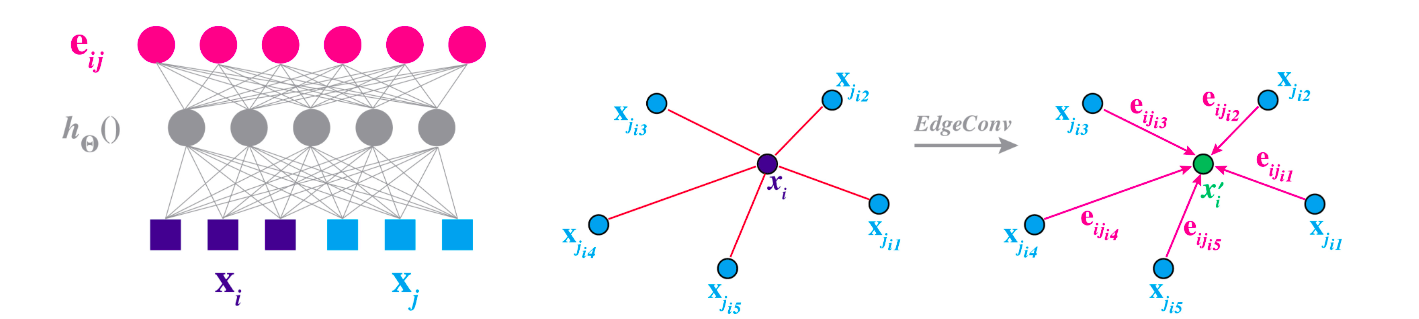
\includegraphics[width=\textwidth]{edgeconv.png}
    \caption{Left: the edge features $e_{ij}$, computed by a fully connected layer. Right: the edge features computed for each edge.~\cite{Wang2019}}
    \label{fig:edgeConvOperator}
\end{figure}

The choice of the $h_{\Theta}$ and $\square$ defines the properties of the EdgeConv operator. The authors of the paper chose an asymmetric edge function:

\begin{equation}\label{eq:edgeconv_h}
h_{\mathbf{\Theta}}\left(\mathbf{x}_{i}, \mathbf{x}_{j}\right)=\bar{h}_{\mathbf{\Theta}}\left(\mathbf{x}_{i}, \mathbf{x}_{j}-\mathbf{x}_{i}\right)
\end{equation}

This function takes into account both the global structure by using the coordinates of $x_i$ and the local structure by using the distances between $x_i$ and its neighbors. This function is easily implemented by an MLP.

As for the aggregation function $\square$ the authors chose the max function:

$$
x_{i}^{\prime}=\max _{j:(i, j) \in \mathcal{E}} e_{i j}^{\prime},
$$

The properties of the EdgeConv operator depend on the choice of the edge and aggregation functions.

Using the $\max$ aggregation achieves permutation invariance with respect to the order of the neighbor points $x_j$.

As for the translation invariance it can seen in equation~\ref{eq:edgeconv_h} that the operator is partially invariant on the translation. It is easy to demonstrate that $h_{\Theta}(x_i - x_j)$ is translation invariant, while $h_{\Theta}(x_i)$ isn't, as shown in equation~\ref{eq:edgeconv_tranls}.

\begin{equation}\label{eq:edgeconv_tranls}
\begin{split}
    \bar{h}_{\mathbf{\Theta}}\left((\mathbf{x}_{j} + T)-(\mathbf{x}_{i} + T), \mathbf{x}_{i} + T \right) = \\
    \theta \cdot ((\mathbf{x}_{j} + T)-(\mathbf{x}_{i} + T)) + \phi \cdot (\mathbf{x}_{i} + T) = \\
    \theta \cdot (\mathbf{x}_{j}-\mathbf{x}_{i}) + \phi \cdot (\mathbf{x}_{i} + T)
\end{split}
\end{equation}


If only the first part is considered then EdgeConv is fully invariant to translation, however the global structure information would be lost: the classification would be based on patches of the point cloud without taking into account the global pose of these patches.

\paragraph{Dynamic graph update}
An important part explored is the dynamic graph computation.
State of the art approaches in graph based network compute the graph at the beginning and then use it throughout the network. DGCNN instead recomputes the graph after each EdgeConv layer: the architecture learns how to construct the graph.
The k-nearest neighbors are found by computing the pairwise distance matrix in feature space.

\paragraph{Architecture and results}

The network architecture used for the evaluation experiments is shown in figure~\ref{fig:DGCNN}. It is composed of 4 EdgeConv layers with skip connections to aggregate multi scale features, obtaining a 512-dimesional point cloud, and a max pooling layer. Then there are multiple fully connected layers. All layers include leaky ReLU as activation function and batch normalization.

\begin{figure}[ht]
    \centering
    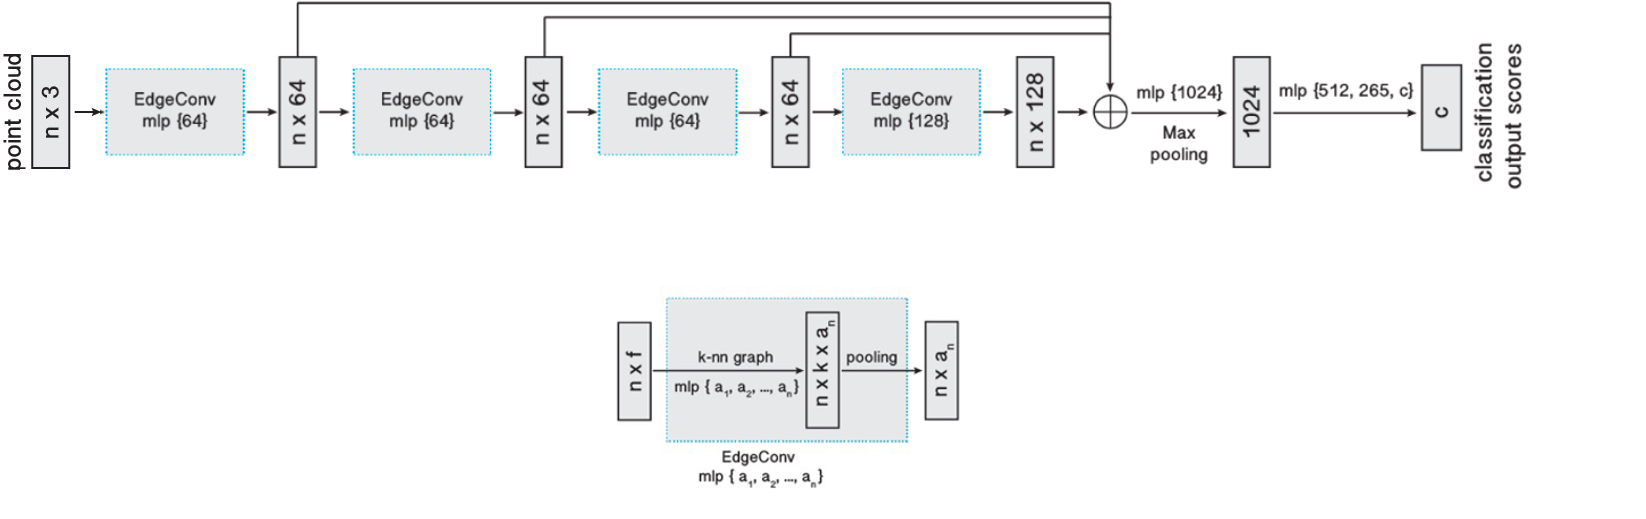
\includegraphics[width=\textwidth]{DGCNN_orig.png}
    \caption{Top: DGCNN network architecture. Bottom: EdgeConv.~\cite{Wang2019}}
    \label{fig:DGCNN}
\end{figure}

The experiments have been performed on ModelNet40, and have been conducted in the same way as PointNet authors did, which have become a standard to have a meaningful comparison between different networks.

The baseline model uses only a fixed graph (no dynamic computation), and uses as edge function $ h_{\Theta}(x_i, x_j)$. With this model an improvement of $\SI{1}{\percent}$ over PointNet++ is achieved.

Multiple experiments have been performed to evaluate how much each part of the model influences the accuracy results, as shown in table~\ref{tab:dgcnn_exp}.
Three improvements to the networks have been tried:

\begin{itemize}
    \item Centralization, which is using explicitly the global information given by the vertex $x_i$ and the distance between its neighbors, by using the edge function ${h}_{\mathbf{\Theta}}\left(\mathbf{x}_{i}, \mathbf{x}_{j}-\mathbf{x}_{i}\right)$.
    \item Dynamic graphs, which is the computation of the neighbors on the features extracted for each EdgeConv layer.
    \item More points, by using 2048 points instead of 1024.
\end{itemize}

\begin{table}[htb]
    \centering
    \caption{CENT denotes centralization, DYN denotes dynamical graph recomputation and MPOINTS denotes experiments with 2,048 points}
    \begin{tabular}{ccccc}
        \hline \text { CENT } & \text { DYN } & \text { MPOINTS } & \text { MEAN CLASS ACCURACY(\%) } & \text { OVERALL ACCURACY(\%) } \\
        \hline x & & & 88.9 & 91.7 \\
        x & x & & 89.3 & 92.2 \\
        x & x & x & 90.2 & 92.9 \\
        \hline
    \end{tabular}
    \label{tab:dgcnn_exp}
\end{table}

It is also worth noticing that DGCNN performs faster than state of the art network such as PointNet++, while keeping the model size relatively small, as shown in table~\ref{tab:dgcnn_exp2}.

\begin{table}[htb]
    \centering
    \caption{Size and time comparison between PointNet, PointNet++ and DGCNN }
    \begin{tabular}{lccc}
        \hline & \text { MODEL SIZE(MB) } & \text { TIME(MS) }  \\
        \hline \text { POINTNET (BASELINE) (QI ET AL. 2017B) } & 9.4 & 6.8  \\
        \text { POINTNET (QI ET AL. 2017B) } & 40 & 16.6 \\
        \text { POINTNET++ (QI ET AL. 2017C) } & 12 & 163.2 \\
        \text { DGCNN (BASELINE) } & 11 & 19.7  \\
        \text { DGCNN } & 21 & 27.2  \\
        \hline
    \end{tabular}
    \label{tab:dgcnn_exp2}
\end{table}

\section{Comparison}

\section{Conclusion}

\bibliographystyle{unsrt}  

\bibliography{references}

\end{document}
